%%% LaTeX Template: Article/Thesis/etc. with colored headings and special fonts
%%%
%%% Source: http://www.howtotex.com/
%%% Feel free to distribute this template, but please keep to referal to http://www.howtotex.com/ here.
%%% February 2011
%%%
%%% Modified October 2015 by CDM

%%%  Preamble
\documentclass[11pt,letterpaper]{article}
\usepackage[margin=1.0in]{geometry}
\usepackage[T1]{fontenc}
\usepackage[bitstream-charter]{mathdesign}
\usepackage[latin1]{inputenc}					
\usepackage{amsmath}						
\usepackage{xcolor}
\usepackage{cite}
\usepackage{hyphenat}
\usepackage{graphicx}
\usepackage{float}
\usepackage{subfigure}
\usepackage{sectsty}
\usepackage[compact]{titlesec} 
\usepackage[tablegrid]{vhistory}
\allsectionsfont{\color{accentcolor}\scshape\selectfont}

%%% Definitions
\definecolor{accentcolor}{rgb}{0.0,0.0,0.5} 
\newcommand{\teamname}{Team Telepresence}
\newcommand{\productname}{Rift Telepresence}
\newcommand{\coursename}{CSE 4317: Senior Design II}
\newcommand{\semester}{Spring 2017}
\newcommand{\docname}{Project Charter}
\newcommand{\department}{Department of Computer Science \& Engineering}
\newcommand{\university}{The University of Texas at Arlington}
\newcommand{\authors}{Cameron Adams \\ John Green \\ Andy Le \\ Clement Olayiwola \\ Ty Simmel}

%%% Headers and footers
\usepackage{fancyhdr}
	\pagestyle{fancy}						% Enabling the custom headers/footers
\usepackage{lastpage}	
	% Header (empty)
	\lhead{}
	\chead{}
	\rhead{}
	% Footer
	\lfoot{\footnotesize \teamname \ - \semester}
	\cfoot{}
	\rfoot{\footnotesize page \thepage\ of \pageref{LastPage}}	% "Page 1 of 2"
	\renewcommand{\headrulewidth}{0.0pt}
	\renewcommand{\footrulewidth}{0.4pt}

%%% Change the abstract environment
\usepackage[runin]{abstract}			% runin option for a run-in title
%\setlength\absleftindent{30pt}			% left margin
%\setlength\absrightindent{30pt}		% right margin
\abslabeldelim{\quad}	
\setlength{\abstitleskip}{-10pt}
\renewcommand{\abstractname}{}
\renewcommand{\abstracttextfont}{\color{accentcolor} \small \slshape}	% slanted text

%%% Start of the document
\begin{document}

%%% Cover sheet
{\centering \huge \color{accentcolor} \sc \textbf{\department \\ \university} \par}
\vspace{1 in}
{\centering \huge \color{accentcolor} \sc \textbf{\docname \\ \coursename \\ \semester} \par}
\vspace{0.5 in}
\begin{figure}[h!]
	\centering
   	
\includegraphics[width=0.60\textwidth]{images/test_image}
\end{figure}
\vspace{0.5 in}
{\centering \huge \color{accentcolor} \sc \textbf{\teamname \\ \productname} \par}
\vspace{0.5 in}
{\centering \large \sc \textbf{\authors} \par}
\newpage


%\vspace{1 in}
%\centerline{January 13th, 2012}
%\newpage

%%% Revision History
\begin{versionhistory}
  	\vhEntry{0.1}{09.29.2016}{CA|JG|AL|CO|TS}{Initial draft}
  	\vhEntry{0.2}{04.25.2017}{CA|JG|AL|CO|TS}{Update draft}
  	\vhEntry{0.3}{04.28.2015}{CA|JG|AL|CO|TS}{Complete draft}
  	%\vhEntry{1.0}{10.20.2015}{AT|GH|CB}{official release}
  	%\vhEntry{1.1}{10.31.2015}{AL}{added customer change requests}
\end{versionhistory}
\newpage

%%% Table of contents
\tableofcontents
\newpage

%%% List of figures and tables (optional)
\listoffigures
%\listoftables
\newpage

%%% Agile project charter sections
\section{Vision}
Create an affordable stereoscopic virtual reality camera system that allows users a "first-hand" view of a place they cannot otherwise go.
\section{Mission}
Our mission is to deliver an affordable, easily mountable, and low profile system with manageably low latency.
\section{Success Criteria}
The necessary results to consider this project a success is the following:

\begin{itemize}
	\item One-to-one head tracking
	\item 3D (Pitch, Yaw, and Roll) camera articulation system
	\item Accurate stereo vision
\end{itemize}
\newpage

%%% Remaining project charter sections
\section{Background}
A stereo camera is a type of camera with two or more lenses with a separate image sensor for each lens. The primary use for a stereoscopic camera comes from the ability to capture three-dimensional images. Stereo cameras may be used for making stereoviews and three-dimensional pictures for movies, or for range imaging. The three-dimensional aspect of the stereo camera is achieved by separating the cameras by a fixed distance. The separation provides a sense of depth when the images are combined. The distance between the lenses in a typical stereo camera is about the distance between one's eyes and is about two and a half inches. The stereo camera has been in use since the 1940's with the Realist format cameras. The technology has progressed significantly over the years. The proliferation of computer vision applications has transformed stereo cameras from an artistic form to a more industrial use. A stereo camera combined with a computer vision algorithm provides the ability to accurately gauge distance and generate depth maps. On the artistic front, the introduction of 3D movies relies entirely on stereo cameras for the non-computer generated content.

A virtual reality headset is comprised of a stereoscopic head-mounted display, providing separate images for each eye, and head motion tracking sensors. The idea of a virtual or augmented reality has motivated attempts to develop a commercial vritual reality headset as early as 1994, Forte VFX1. The goal of creating an immersive virtual reality experience for the wearer has been hindered by the lack of computational power needed to drive such a device. The cost to develop and operate a virtual reality headset limited the potential applications to simulators and training facilities. This cost limitation changed in 2012 with the funding campaign that began the Oculus Rift. Over a four year period, many developments were made in the consumer virtual reality headset market. The concurrent development of the HTC Vive to compete with the Oculus has left the consumer market with two functional and cheap virtual reality headsets.
\section{Related Work}
Similar to the awareness the public had of augmented reality before Pok\'{e}mon Go increased the awareness, virtual reality was around for many decades. Nowadays, virtual reality has been increasing the awareness of the public because commercial products are being developed and sold. A head mounted display is usually used to experience the virtual world. In a recent development of a virtual reality camera, the Orah 4i will make it possible to live stream video footage to a head mounted display or to a mobile phone that can offer virtual reality options. The Orah 4i has four image sensors with fisheye lenses to be able to capture an output with a 360\textdegree field of view. A stitching box is included with the product to live stream the video footage with high quality. Even before the development of Orah 4i, companies sold 360\textdegree cameras that supported virtual reality such as Nokia, Samsung, and Vuze. Another camera besides the 360\textdegree field of view in the market is the stereo camera. Stereo cameras capture the depth of the three-dimensional images taken from the camera. Unlike the 360\textdegree cameras, stereo cameras have a field of view less than 180\textdegree, and it has two image sensors. The ZED camera is an example of a stereo camera where the depth is captured in the images.
\section{System Overview}
The Camera System handles three primary tasks. The motor controller board receives signals from the Processing System. The control board then orients the gimbal to the angles specified by the signals. For the final task, the cameras capture stereo video and pass the video to the Processing System. The Processing System serves as an intermediary between the Camera System and Virtual Reality System. The two functionalities are processing the video and translating the head tracking data. The final system is the Virtual Reality System. This system is responsible for the stereo display of the video and the capture of the raw head tracking data.

\begin{figure}[h!]
	\centering
 	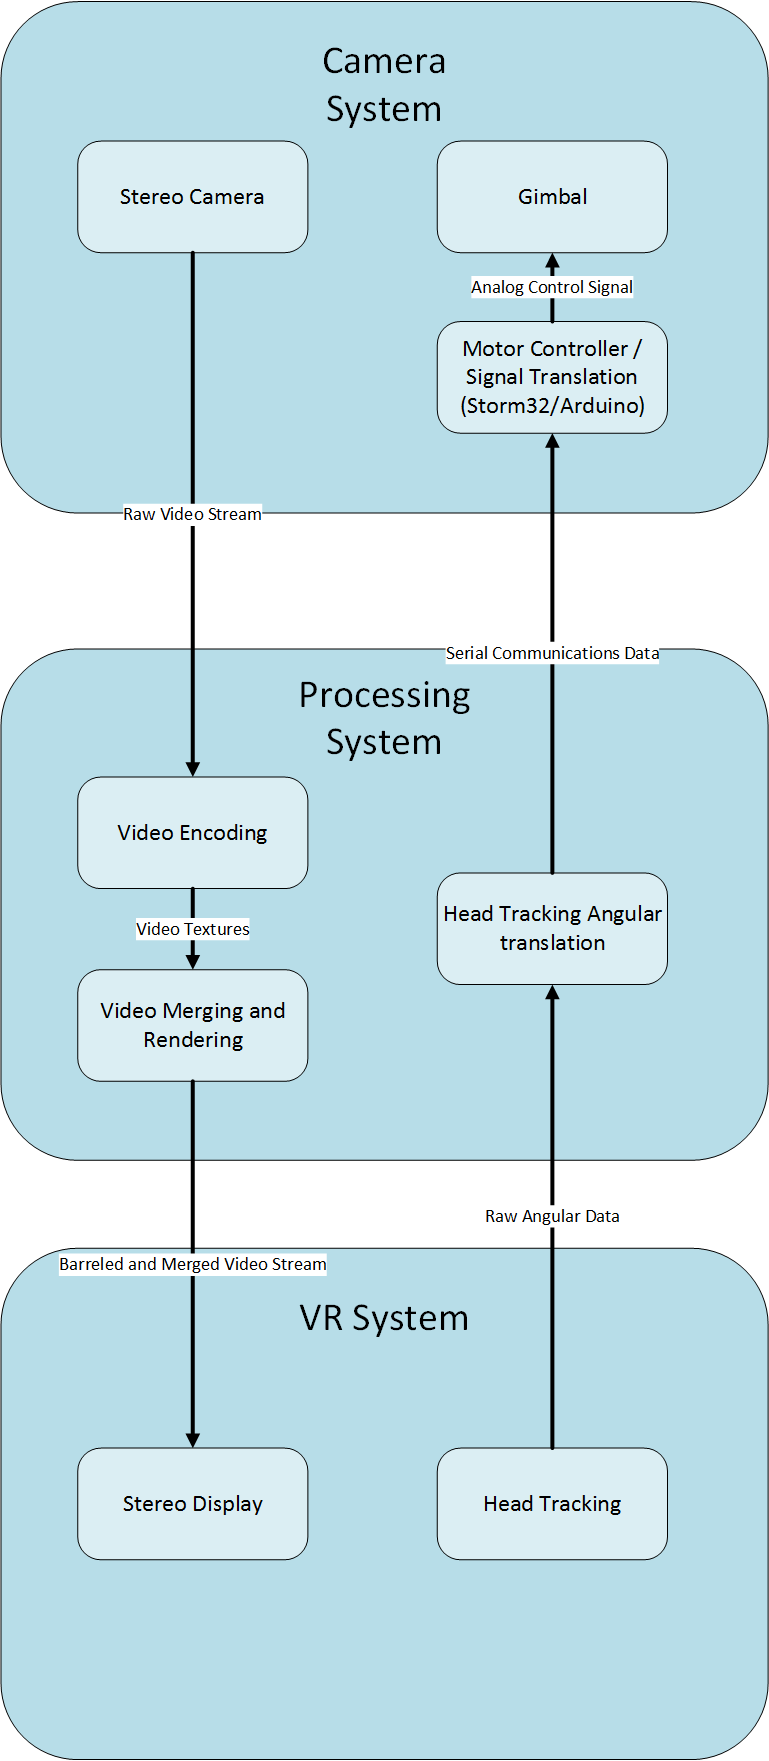
\includegraphics[width=0.27\textwidth]{images/Overview}
 \caption{System architecture}
\end{figure}

\section{Roles \& Responsibilities}
Cameron Adams: I have a good understanding of design concepts and will focus primarily on the virtual reality headset to camera system communication.
\\\\
John Green: I have a good understanding of mechanical design concepts in relation to servos, control arms, and pulley systems. My strength is in low level computer system to system interactions. My focus will be gimbal design and translation
\\\\
Andy Le: I have an understanding of software testing and I will focus on the data transfer between the virtual reality headset and camera.
\\\\
Ty Simmel: I have a strong background in circuit design and will primarily focus on powering the system,  embedded programming,  and design aesthetics.
\\\\
Clement Olayiwola:   I have a passion for documentation, testing, project research, and project analysis. I will focus mainly on video communication.
\\\\
\section{Facilities \& Equipment}
The following are needed to develop the product:

\begin{itemize}
	\item Lab space
	\item Desktop computer with a dedicated graphics card
	\item 3D printer
	\item Oculus Rift
\end{itemize}
\section{Cost Proposal}
\subsection{Preliminary Budget}
The preliminary budget consists of \char36 800 grant provided by the university.

\subsection{Current \& Pending Support}
No other funding has been pursued as of this time.
\section{Documentation \& Reporting}
\subsection{Project Charter}
The project charter is to be revisited and maintained as the project requirements develop.

\subsection{Product Backlog}
Prioritized list of tasks to be completed. This will be rigorously maintained and updated as the project develops.

\subsection{Sprint Planning}
Sprints are to be voted on and tasks assigned according to each member's skills and preferences.

\subsubsection{Sprint Goal}
As there will be no definitive team manager, the team will vote on goals.

\subsubsection{Sprint Backlog}
The sprint backlog tasks are to be pulled from the highest remaining priority backlog tasks. Lower priority tasks with dependencies will be pulled and assigned as needed.

\subsubsection{Task Breakdown}
The team will vote on each team member's individual tasks every two weeks.

\subsection{Sprint Burndown Charts}
Burndown charts are to be revisited every two weeks.

\begin{figure}[h!]
    \centering
    
\includegraphics[width=0.5\textwidth]{images/test_image}
    \caption{Example sprint burndown chart}
\end{figure}

\subsection{Sprint Retrospective}
Weekly meetings are in order to discuss the direction of the product development. As development continues, the team will update policies and procedures to ensure maximum working efficiency.

\subsection{Individual Status Reports}
Weekly status reports are to be given by each team member. These may align with the beginning or end of a sprint, or occur mid-sprint.

\subsection{Engineering Notebooks}
The group will have weekly sign offs by team members ensuring that each member's respective work has been documented.

\subsection{Closeout Materials}
Hardware includes the mounted stereoscopic camera set. The group will provide software which allows communication between a PC and a virtual reality headset. Full documentation will be provided. An operational reference guide will be provided for the software needed to run the virtual reality system. A demonstration video is to be provided.

\subsubsection{System Prototype}
No system prototype is available at this point.

\subsubsection{Project Poster}
The team will develop a project poster when the system requirements become more clear.

\subsubsection{Web Page}
The group has agreed against a webpage as it would not serve any practical benefits to the system.

\subsubsection{Demo Video}
A system demonstration video is to be released once a physical prototype is available.

\subsubsection{Source Code}
While the project is software and hardware extensive, there should be nominal source code involved in engineering the system. Team-developed codes will mainly be used to track the gimbal to a virtual reality headset's accelerometer. All source code should remain neat, concise, and efficient.

\subsubsection{Source Code Documentation}
The code's developer should also provide documentation over the code according to standard professional practices.

\subsubsection{Hardware Schematics}
Hardware schematics will be continuously updated as project development continues.

\subsubsection{CAD files}
There will be CAD files which document hardware designs.

\subsubsection{Installation Scripts}
The team will be performing on-site deployment.

\subsubsection{User Manual}
A brief user manual is to be provided which will map the controls relative to the setup of the virtual reality headset and the general warnings associated with virtual reality headset use.

\newpage

%%% References
\bibliographystyle{plain}
\bibliographystyle{reference/IEEEtran_custom}
\bibliography{reference/refs}{}

\end{document}